\documentclass[10pt]{article}
\usepackage{xcolor}

\usepackage{listings}

\usepackage{geometry}
% NCE maximal width is 15 cm
\geometry{paperwidth=3.5in, paperheight=3.5in, top=0pt, bottom=0pt, right=0pt, left=0pt}
\usepackage{tikz}
\usetikzlibrary{arrows, calc, patterns, decorations.pathmorphing, fit, positioning, shapes.misc}


\def\grid{6}        % grid size (mm)
\def\laneGap{2}     % gap between lanes (mm)
\def\ellipsisGap{5} % gap to last lane (mm)

\begin{document}
\begin{tikzpicture}

    %--------------------------------------------------------
    % Sparse
    %--------------------------------------------------------
    \node (block_sparse) at (0, 0){
        \begin{tikzpicture}
            % Draw first lanes
            \pgfmathtruncatemacro{\laneHeight}{8 * \grid}
            \foreach \j in {0,...,1} {
                \pgfmathtruncatemacro{\laneStart}{\j * (\laneGap + \grid)}
                
                \draw[step=\grid mm] (\laneStart mm, 0) grid (\laneStart mm + \grid mm, \laneHeight mm);
                
                % Draw labels
                \foreach \i in {0,...,7} {
                    \pgfmathtruncatemacro{\index}{\j + (32 * (7 - \i))}
                    
                    \node at ({\laneStart mm + (\grid mm / 2)},  {\grid mm * (\i + 0.5)}) {$i_{\index}$};
                }
            }
            
            % Draw last lane
            \pgfmathtruncatemacro{\lastLaneStart}{(2 * (\laneGap + \grid)) + \ellipsisGap}
            \draw[step=\grid mm] (\lastLaneStart mm, 0) grid (\lastLaneStart mm + \grid mm, \laneHeight mm);
            
            % Draw labels
            \foreach \i in {0,...,7} {
                \pgfmathtruncatemacro{\index}{31 + (32 * (7 - \i))}
                
                \node at ({\lastLaneStart mm + (\grid mm / 2)},  {\grid mm * (\i + 0.5)}) {$i_{\index}$};
            }

        \end{tikzpicture}
    };
    
    %--------------------------------------------------------
    % Delayed
    %--------------------------------------------------------
    \node (block_delay) at (50mm, 0){
        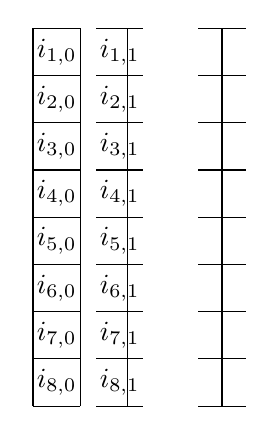
\begin{tikzpicture}
            % Draw first lanes
            \pgfmathtruncatemacro{\laneHeight}{8 * \grid}
            \foreach \j in {0,...,1} {
                \pgfmathtruncatemacro{\laneStart}{\j * (\laneGap + \grid)}
                
                \draw[step=\grid mm] (\laneStart mm, 0) grid (\laneStart mm + \grid mm, \laneHeight mm);
                
                % Draw labels
                \foreach \i in {0,...,7} {
                    \pgfmathtruncatemacro{\topDownI}{8 - \i}
                    \node at ({\laneStart mm + (\grid mm / 2)},  {\grid mm * (\i + 0.5)}) {$i_{\topDownI, \j}$};
                }
            }
            
            % Draw last lane
            \pgfmathtruncatemacro{\lastLaneStart}{(2 * (\laneGap + \grid)) + \ellipsisGap}
            \draw[step=\grid mm] (\lastLaneStart mm, 0) grid (\lastLaneStart mm + \grid mm, \laneHeight mm);

        \end{tikzpicture}
    };

\end{tikzpicture}
\end{document}
